% ****** Start of file apssamp.tex ******
%
%   This file is part of the APS files in the REVTeX 4.2 distribution.
%   Version 4.2a of REVTeX, December 2014
%
%   Copyright (c) 2014 The American Physical Society.
%
%   See the REVTeX 4 README file for restrictions and more information.
%
% TeX'ing this file requires that you have AMS-LaTeX 2.0 installed
% as well as the rest of the prerequisites for REVTeX 4.2
%
% See the REVTeX 4 README file
% It also requires running BibTeX. The commands are as follows:
%
%  1)  latex apssamp.tex
%  2)  bibtex apssamp
%  3)  latex apssamp.tex
%  4)  latex apssamp.tex
%
\documentclass[%
 reprint,
% draft,
%superscriptaddress,
%groupedaddress,
%unsortedaddress,
%runinaddress,
%frontmatterverbose, 
%preprint,
%preprintnumbers,
%nofootinbib,
%nobibnotes,
%bibnotes,
 amsmath,amssymb,
 aps,
%pra,
%prb,
%rmp,
%prstab,
%prstper,
%floatfix,
]{revtex4-2}

\usepackage{graphicx}% Include figure files
\usepackage{mathtools}
\usepackage{dcolumn}% Align table columns on decimal point
\usepackage{bm}% bold math
\renewcommand\vec\bm  % Bold vector instead of arrow
\DeclareMathOperator\sign{sign}
\usepackage{braket}
\usepackage{subcaption}
\usepackage{microtype}
\usepackage{hyperref}% add hypertext capabilities
%\usepackage[mathlines]{lineno}% Enable numbering of text and display math
%\linenumbers\relax % Commence numbering lines

%\usepackage[showframe,%Uncomment any one of the following lines to test 
%%scale=0.7, marginratio={1:1, 2:3}, ignoreall,% default settings
%%text={7in,10in},centering,
%%margin=1.5in,
%%total={6.5in,8.75in}, top=1.2in, left=0.9in, includefoot,
%%height=10in,a5paper,hmargin={3cm,0.8in},
%]{geometry}


\usepackage{xcolor}
\newcommand{\cbox}[2][yellow]{%
  \colorbox{#1}{\parbox{\dimexpr\linewidth-2\fboxsep}{\strut #2\strut}}%
}
\newcommand{\todo}[2][orange]{\hfill\break{\bfseries\cbox[#1]{#2}}\break}

\begin{document}

\preprint{APS/123-QED}

\title{Nernst effect from conformal anomaly in tilted Weyl semimetals}% Force line breaks with \\

\author{Thorvald Molthe Ballestad}
\email{thorvald.tb@gmail.com}
\noaffiliation
% \affiliation{%
%   Center for Quantum Spintronics, Department of Physics,Norwegian University of Science and Technology, Trondheim, Norway.
% }%

\author{María A. H. Vozmediano}%
\affiliation{%
  Materials Science Factory, Instituto de Ciencia de Materiales de Madrid, CSIC, Cantoblanco, 28049 Madrid, Spain.}

\author{Alberto Cortijo}%
\affiliation{%
  Materials Science Factory, Instituto de Ciencia de Materiales de Madrid, CSIC, Cantoblanco, 28049 Madrid, Spain.}

\author{Alireza Qaiumzadeh}%
\email{alireza.qaiumzadeh@ntnu.no}
\affiliation{%
  Center for Quantum Spintronics, Department of Physics,Norwegian University of Science and Technology, Trondheim, Norway.
}%

% \collaboration{MUSO Collaboration}%\noaffiliation

% \author{Charlie Author}
%  \homepage{http://www.Second.institution.edu/~Charlie.Author}
% \affiliation{
%  Second institution and/or address\\
%  This line break forced% with \\
% }%
% \affiliation{
%  Third institution, the second for Charlie Author
% }%
% \author{Delta Author}
% \affiliation{%
%  Authors' institution and/or address\\
%  This line break forced with \textbackslash\textbackslash
% }%

% \collaboration{CLEO Collaboration}%\noaffiliation

\date{\today}% It is always \today, today,
             %  but any date may be explicitly specified

\begin{abstract}
  We calculate a Nernst current in tilted Weyl semimetals using the Kubo formalism.

% \begin{description}
% \item[Usage]
% Secondary publications and information retrieval purposes.
% \item[Structure]
% You may use the \texttt{description} environment to structure your abstract;
% use the optional argument of the \verb+\item+ command to give the category of each item.
% \end{description}
\end{abstract}

%\keywords{Suggested keywords}%Use showkeys class option if keyword
                              %display desired
\maketitle

%\tableofcontents
\section{Calculation\label{sec:calculation}}
\subsection{Setup and response}
Consider the Hamiltonian
\begin{equation}
  \label{eq:hamiltonian}
  H^s = s v_F \vec{\sigma} \cdot \vec{p} + v_F \vec{t}^s \vec{p},
\end{equation}
with \( s = \pm 1 \) the chirality of the cone, \( v_F \) the Fermi velocity, \( \vec{\sigma} \) the Pauli matrix vector, \( \vec{p} \) the momentum operator and \( \vec{t}^s \) the \emph{tilt vector}.
For inversion symmetric systems \( \vec{t}^s = s \vec{t} \), while broken inversion symmetry we consider \( \vec{t}^s = \vec{t} \)
\footnote{We here chose the ``antisymmetric'' version for the broken inversion symmetry, where the cones tilt in the same direction with the same magnitude.
Of course, many other choices also break inversion symmetry.}.

...
The response from the Kubo formalism is thus
\begin{equation}
  \label{eq:kubo-response}
  \begin{multlined}
    \chi^{ij}(\omega, \vec{q}) = \frac{-i v_F}{\mathcal{V}}
    \int \mathrm{d} t
    e^{i \omega t}
    \int\limits_{-\infty}^0 \mathrm{d} t'
    \Theta(t)\\
    \times
    \Braket{\left[J^i(t, \vec{q}), T^{j0}(t', -\vec{q})\right]},
  \end{multlined}
\end{equation}
where \( \hbar = 1 \).
The charge current operator
\begin{equation}
  \label{eq:current-op}
  \vec{J} = e v_F (s \vec{\sigma} + \vec{t}^s).
\end{equation}
For the energy-momentum tensor choose
\footnote{TODO: add some discussion here or in appendix}
\begin{equation}
  \label{eq:energy-momentum-tensor}
  T^{\mu\nu} =
  \frac{i}{2} (
  \phi^{\dagger} \tilde{\sigma}^{\mu} \partial_{\nu} \phi
  -\tilde{\sigma} ^{\mu} \phi^{\dagger} \partial_{\nu} \phi
  -\eta^{\mu \nu} \mathcal{L}
  ),
\end{equation}
where we have defined the modified Pauli matrices \( \tilde{\sigma} ^{\mu} = \sigma^{\mu} + (t^s)^{\mu} \) with \( (t^s)^{\mu} = (0, \vec{t}^s) \).

For concreteness, we will, without loss of generality, consider the geometry \( \vec{J} \parallel \hat{x}, -\nabla T \parallel \hat{y}, \vec{B} \parallel \hat{z} \).
We separate between \emph{perpendicular} and \emph{parallel} tilt, with the former being \( \vec{t} \perp \vec{B}
\) and the latter \( \vec{t} \parallel \vec{B} \).
In the current work we have furthermore restricted the perpendicular tilt to be parallel to the current, i.e. \( \vec{t}_{\perp} = t_x \hat{x} \).

\subsection{Landau levels}
The Landau levels can be shown to be
\begin{equation}
  \label{eq:eigenlevels}
  E_{k_z m s} =
  \begin{cases}
    t_z^s v_F k_z + \sign(m) v_F \alpha \sqrt{2 e B \alpha M + k_z^2} & m \neq 0,\\
    t_z^s v_F k_z - s \alpha v_F k_z & m = 0,
  \end{cases}
\end{equation}
where we have defined the \emph{squeezing factor} \( \alpha = \sqrt{1 + t_x^2} \).
The eigenstates in the position basis are
\begin{equation}
  \label{eq:eigenstates}
  \phi(\vec{r}) = \sqrt{\alpha} e^{\theta / 2 \sigma_x} \frac{e^{i k_x x + ik_z z }}{\sqrt{L_{x} L_{z}}} e^{- \frac{1}{2} \chi^2}
  \begin{pmatrix}
    a_{k_z m s} H_{M-1} (\chi)\\
    b_{k_z m s} H_M (\chi)
  \end{pmatrix},
\end{equation}
where we defiend the dimesionless quantity \( \chi = \sqrt{\alpha} \frac{y-k_{x}l_B^2}{l_{B}} + \frac{t_x^s l_B}{\sqrt{\alpha} v_{F}} E^0_{m, \alpha B} \).

In the local limit \( \vec{q} \to 0 \) we find
\begin{align}
  \label{eq:1}
  J_{k_z m n s} &= \Gamma_{k_z m n s} s v_F e ( \alpha_{k_z m s } \delta_{M-1, N} + m \leftrightarrow n),\\
  T_{k_z m n s}^{0y} &=
                       \begin{multlined}[t]
                         \frac{i s \Gamma_{k_z m n s}}{4} (E_{k_z m s} + E_{k_z n s} - 2 \mu )\\
                         \times (\alpha_{k_z m s} \delta_{M-1, N} - m \leftrightarrow n),
                       \end{multlined}
\end{align}
where \( m \leftrightarrow n  \) represents the preceding term under the interchange of \( m,n \), and we have defined \( \Gamma_{\kappa_z m n s} = \left[(\alpha_{k_z m s}^2 + 1) (\alpha{k_z n s}^2 + 1)\right]^{-\frac{1}{2}} \).

\section{Results\label{sec:results}}
We find the response in the limit \( T\to 0 \) and with zero chemical potential \( \mu = 0 \),
\begin{equation}
  \label{eq:response-w-dimensions}
  \lim_{\omega \to 0} \lim_{\vec{q} \to 0}
  \chi^{xy} =
  \gamma_{N} \frac{e^2 v_F B}{(2\pi)^2},
\end{equation}
where \( \gamma_N \) is a term generally depending on the number of Landau levels included in the sum, and the tilting vector \( \vec{t} \).

The case of no tilt was first solved by \textcite{chernodubGenerationNernstCurrent2018} and then using Kubo formalism by \textcite{arjonaFingerprintsConformalAnomaly2019}.
We have simplified their computation and found an analytical expression for the prefactor, with the iterative expression
\begin{equation}
  \label{eq:2}
  \gamma_{N} - \gamma_{N-1} = \frac{1}{4} \left[ 1 + 2 N \left\{ 1 - (1+N) \log \left(1 + \frac{1}{N}\right) \right\} \right],
\end{equation}
for \( N>0 \), and \( \gamma_0 = \frac{1}{4} \).
It can be shown that
\begin{multline}
  \label{eq:4}
  \gamma_N = \gamma_0 + \frac{1}{12} \Big(
    6 \zeta ^{(1,0)}(-2,N+1)
    -6 \zeta ^{(1,0)}(-2,N+2)\\
    +6 \zeta^{(1,0)}(-1,N+1)
    + 6 \zeta^{(1,0)}(-1,N+2)\\
    +12 \log (\xi)
    +3 N^2
    +6 N
    -1
  \Big),
\end{multline}
where \( \xi \approx  1.28243 \) is Glaisher's constant.


The contribution from the cone with chirality \( s = -1 \) can be found from the result of the positive chirality cone.
In the case of perpendicular tilt, they are exactly the same.
In the case of parallel tilt, it depends on the symmetry of the tilt.
For systems with broken inversion symmetry, the response from the two cones are the same.
On the other hand, for inversion symmeric systems, the contribution form the cone with chirality \( s=-1 \) is the same as that of the \( s=+1 \) cone at the opposite tilt \( t_z \to - t_z \).
Therefore, it is useful to separate the contribution into even and odd components, for finding the total contribution from the two cones combined.
For some contribution \( \gamma(t_{x /z}) \), we define
\begin{align}
  \gamma_{\text{even}}(t_{x/z}) &= \frac{\gamma(t_{x/z}) + \gamma(-t_{x/z})}{2}\label{eq:132},\\
  \gamma_{\text{odd}}(t_{x/z}) &= \frac{\gamma(t_{x/z}) - \gamma(-t_{x/z})}{2}\label{eq:133}.
\end{align}
All results will be given in terms of these components, at \( t_{x /y} > 0 \).

\subsection{Perpendicular tilt}
We found the response to be even in \( t_x \), and independent of the chirality \( s \).
The response was solved numerically and is shown in figure \ref{fig:contribtx}.
As the tilt is increased, the response is gradually reduced.

\subsection{Parallel tilt}
In the Type-I regime, the response has an extra term compared to the untilted case, \( \gamma_N = \gamma^{0}_{N} + \gamma_{\text{div}, N} \), with \( \gamma_N^0 \) the untitled response and
\begin{equation}
  \label{eq:5}
  \gamma_{\text{div}, N} =  -2 \sum\limits_{i=0}^N \int \mathrm{d} \kappa_z \xi(\kappa_z) \kappa_z t_z \alpha_{\kappa_z m s}^2\Big|_{\overset{m=i+1}{n=-i}} ,
\end{equation}
where \( \kappa_z = \sqrt{2 e B} k_{z} \) and
\begin{equation}
  \label{eq:3}
  \xi(\kappa_z) = \frac{[n_{\kappa ms} - n_{\kappa ns}]
  }{
    \left[ (\alpha_{\kappa ms}^2 + 1) (\alpha_{\kappa ns}^2 + 1) \right]
    (\epsilon _{\kappa m s} - \epsilon _{\kappa n s})^2
  }.
\end{equation}
This contribution has a UV divergence, and we introduce the momentum cutoff \( \Lambda \).
\todo{Add discussion about linear model and cutoff}
The integral was solved analytically, and the contribution from each term found to be
\begin{widetext}
  \begin{equation}
    \label{eq:6}
    \gamma_{\text{div}, N} - \gamma_{\text{div}, N-1} =
    \frac{t_z}{4}
    \Bigg\{
    \Lambda \left(\sqrt{1 + \Lambda^2 + m} - \sqrt{\Lambda^2 + m} \right)
    + m \tanh^{-1} \left[\frac{\Lambda}{\sqrt{\Lambda^2 + m} }\right]
    - (m+1) \tanh^{-1} \left[ \frac{\Lambda}{\sqrt{1 + \Lambda^2 + m }} \right]
    \Bigg\}.
  \end{equation}
\end{widetext}
In the case of Type-II systems, the calculation is more involved, because of the Landau levels crossing the Fermi surface.
This gives both intraband and interband transitions, and the integration limits are more involved.
The zeroth transition \( 0 \to 1 \) was found to be
\begin{equation}
  \label{eq:7}
  \frac{\sign(t_z)}{2}
  \left( |t_z| \sinh^{-1} \left(\frac{1}{\sqrt{t_{z}^2 -1} }\right) -1 \right).
\end{equation}
The higher order contributions were also computed analytically, with very lengthy expressions.
A schematic summary of all the contributions are given in figure \ref{fig:schematic_tz}.


\begin{figure}[p]
\subcaptionbox{Type-I}{
    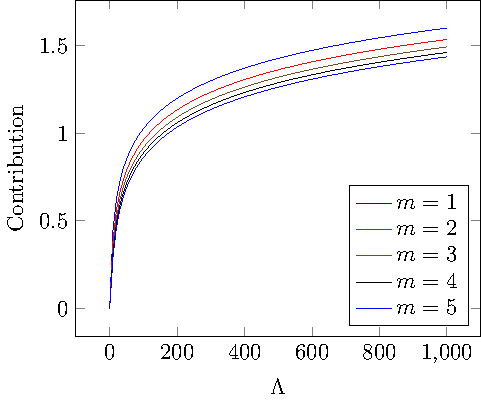
\includegraphics[width=.8\columnwidth]{figures/divergentContribCutoff}
}
\subcaptionbox{Type-II inter band}{
    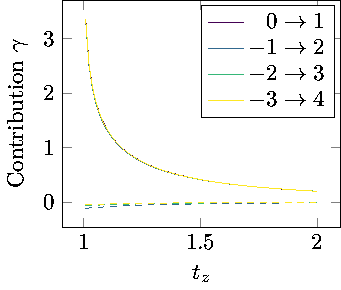
\includegraphics[width=.8\columnwidth]{figures/tzcontribtypeii}
}
\subcaptionbox{Type-II intraband}{
    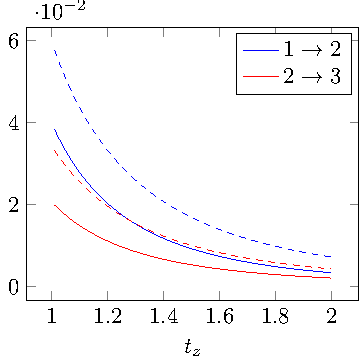
\includegraphics[width=.8\columnwidth]{figures/tzcontribtypeii_intraband}
}
\caption{Contributions in for parallel tilt, for Type-I and Type-II.
  Components even in \( t_z \) are given in solid line, while odd components are given in dashed line.
}
\end{figure}

\begin{figure*}[p]
  \centering
  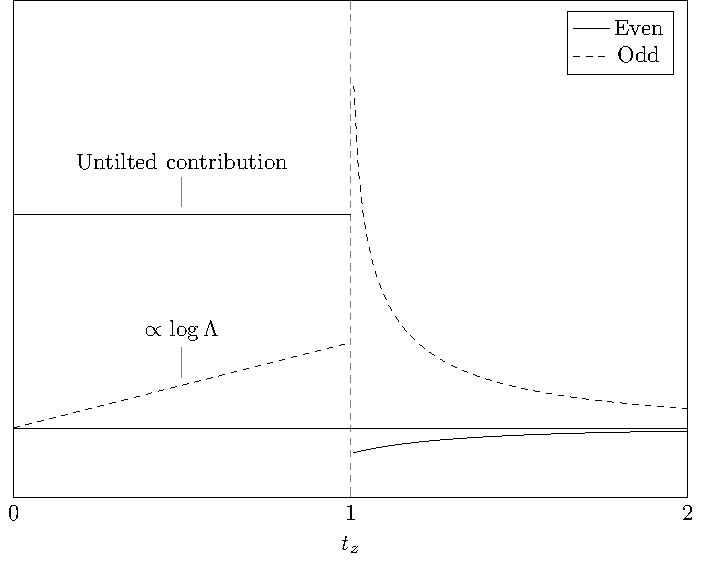
\includegraphics[width=.8\textwidth]{figures/schematic_tz}
  \caption{Schematic summary of the contributions for perpendicular tilt \(t_z \). Shown is the even (solid) and odd (dashed) parts as functions of \(t_z\).}
  \label{fig:schematic_tz}
\end{figure*}

\begin{figure*}[p]
  \centering
  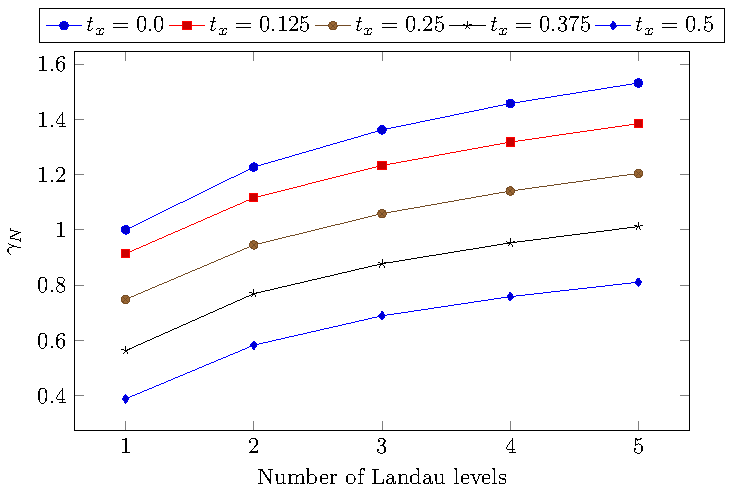
\includegraphics[width=.8\textwidth]{figures/contribtx}
  \caption{\label{fig:contribtx}Contribution as a function of number of Landau levels N for various values of \(t_x\).}
\end{figure*}


% The \nocite command causes all entries in a bibliography to be printed out
% whether or not they are actually referenced in the text. This is appropriate
% for the sample file to show the different styles of references, but authors
% most likely will not want to use it.
\nocite{*}

% \bibliography{apssamp}% Produces the bibliography via BibTeX.
\bibliography{Master.bib}% Produces the bibliography via BibTeX.

\end{document}
%
% ****** End of file apssamp.tex ******
